\section{Path sampling}

\begin{frame}
    \frametitle{Levy construction}
    \framesubtitle{}
  
    \begin{columns}
      \begin{column}{0.4\textwidth}
        \begin{itemize}[itemsep=0.5em, label=$\bullet$]
            \item studio mossa per $x_k$
            \item posizioni adiacenti: $x_1$, $x_2$
            \item intervalli temporali: $\Delta t_1$, $\Delta t_2$
        \end{itemize}

      \end{column}
      
      \begin{column}{0.6\textwidth}
        $$
            \pi^{free}\left(x_k | x_1,\,x_2\right)\,\propto\,\rho^{free}\left(x_1,\,x_k,\,\Delta t_1\right)\rho^{free}\left(x_,\,x_2,\,\Delta t_2\right)
        $$

        \vspace{12pt}
        \centering
        Distribuzione delle mosse gaussiana:
        $$
            \left<x_k\right>\,=\,\frac{\Delta t_2 x_1\,+\,\Delta t_1 x_2}{\Delta t_1\,+\,\Delta t_2}
        $$
        $$
            \sigma\,=\,\left(\frac{1}{\Delta t_2}\,+\,\frac{1}{\Delta t_1}\right)^{-1/2}
        $$
        
      \end{column}
    \end{columns}
  
\end{frame}


\begin{frame}
    \frametitle{Esempio di cammini liberi}
    \framesubtitle{}
  
    \begin{figure}
        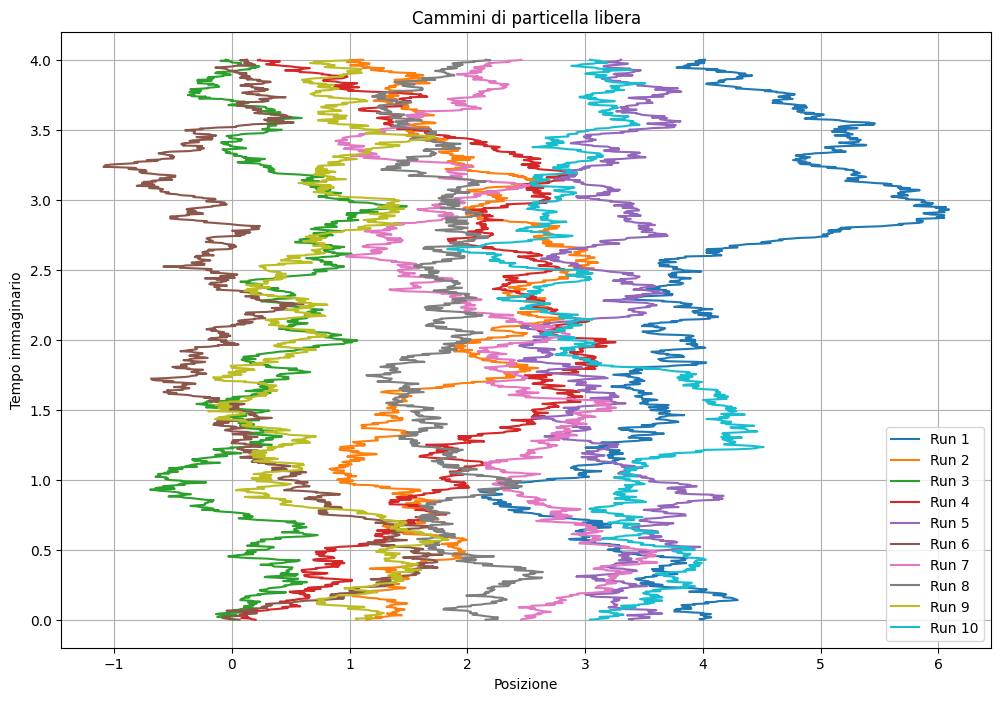
\includegraphics[width=0.55\textwidth]{Immagini/esempioPath.png}
        \caption{Cammini costruiti con ricostruzione di Levy}
    \end{figure}
  
\end{frame}
